\documentclass[5p,authoryear]{elsarticle}
\makeatletter 
\def\ps@pprintTitle{%
 \let\@oddhead\@empty
 \let\@evenhead\@empty
 \let\@evenfoot\@oddfoot} % Supprimer le bas de page ELSEVIER
\makeatother
\usepackage[utf8]{inputenc} % En unicode
\usepackage[T1]{fontenc}
\usepackage[english]{babel}
\usepackage[babel=true]{csquotes} % permet de faire \enquote{a} (« a »)
\usepackage[fleqn]{amsmath} % pour certains signes mathématiques
\usepackage{amsthm} % Pour \begin{gather}
\usepackage{booktabs} % pour \toprule (un style de tableau)
\usepackage{multirow} % Pour colonnes multiples des tableaux
\usepackage{amssymb} % Pour \leqslant (<=, >=)
\usepackage{float}
\usepackage{hyperref} % 
\usepackage[english]{cleveref} 




%\bibliographystyle{elsarticle-num}
\bibliographystyle{elsarticle-harv}

\usepackage{fancyhdr}
\pagestyle{fancy}
\lhead{MSDS 458 - SEC 56}
\rhead{Lee, J.}

\begin{document}

\begin{frontmatter}

\title{Sign Language for Robots: Computer Vision –\\ A Convolutional Neural Network Analysis}
% Research Assignment 2
%% Group authors per affiliation:
\author{Jason Lee}
\address{Northwestern University, SPS \\Artificial Intelligence and Deep Learning \\2019FA MSDS 458-56}


\begin{abstract}

Artificial neural networks are extremely powerful algorithms that are able to solve very complicated problems. This paper investigates the building and tuning of convolutional neural networks (CNNs), which are commonly used to solve computer vision problems. It is important to understand when and how to utilize the various techniques available when building deep (multiple hidden layers) neural networks. This analysis focuses on the effects that hyperparameter settings and network topologies have on the total training time and final out-of-sample prediction accuracy for a CNN. These CNNs will be built to decipher the alphabet in sign language.

%%\footnotemark{}.

\end{abstract}


\begin{keyword}
Convolutional Neural Networks \sep Deep Learning \sep Computer Vision \sep Keras\end{keyword}

\end{frontmatter}

%% \footnotetext{Travail encadré de recherche. Il s'agit d'un travail de trois mois, par équipe de 4 à 5 étudiants, effectué durant le long du deuxième semestre de M1 informatique, à l'université Toulouse 3 — Paul Sabatier.}


%\linenumbers
\section{Introduction}\label{introduction}

Computer vision has been dominating headlines within the artificial intelligence community over the last several years as it is one of the most applicable and interesting problems to be solved in data science. Facial recognition to help tag photos, interpreting and translating handwritten notes and messages to word documents, deciphering between digits written on a bank check, or real-time player and ball identification in professional sporting events are all real-world examples of computer vision being utilized today. 

Humans are masters when it comes to image recognition. It is one of the first problems babies solve as young as 4-6 months old \citep{baby}. On the other hand, image recognition was one of the most challenging problems for a computer to solve. It is a tough pill to swallow knowing that a 4-month-old baby is better than many computer algorithms when it comes to recognizing faces. However, with computing power increasing, computer vision is possible by using deep artificial neural networks.

For image recognition, using a dense, or fully connected, neural network is similar to breaking a picture up into individual pixels, tossing them into a bag, shaking it up, dumping them onto a table, and trying to interpret what image this mess of pixels represents. As was shown in the previous study, simple neural networks are able to predict reasonably well what the jumbled pixels collectively represent in a very basic classification problem \citep{jason}. However, the location and context of the different shapes and colors in the image are completely lost with this approach causing these models to fail completely with more complicated problems. 

This is where convolutional neural networks come in. Convolutional neural networks are one of the most powerful types of algorithms that are consistently performing at the top of all the leaderboards in data science tournaments. They have the ability to take in sections of an image capturing key object groupings and colors within the picture. 

Similar to basic neural networks, a convolutional neural network is a mathematically dependent model that receives input data and produces an output based on strict mathematical rules. These models are able to improve, or learn, over the course of their training time as internal weights are updated in a feedback loop. The performance of a deep learning model is dependent on how each layer is stacked, how the hyperparameters are tuned, and what training, validation, and testing datasets are used. 

Neural networks have a tendency to overfit to the training dataset. This causes neural networks to learn features that are not actually useful when predicting on new samples. Failure to understand how a deep neural network learns could have catastrophic consequences in the real world. There have been citizens, like Eric Loomis of Wisconsin, sentenced to much harsher prison times because of potentially biased black-box models \citep{prison}. Understanding what each layer is learning from the input data and how the layer is contributing to the model holistically will enable the data scientist to build and deploy trustworthy deep learning models in the real world, which is the aim of this study.

The specific purpose of this analysis is three-fold: 1 – Determine the proper way to construct a trustworthy deep neural network. 2 – Explore the effects neural network topology and hyperparameter settings have on the convolutional neural network’s training time and overall performance. 3 – Generate a reproducible Python prediction model to easily share with colleagues. 



\subsection{Sign Language Recognition} \label{sign}

To accomplish the goals of this study, the American Sign Language alphabet will be used for the computer vision models. A sample image of each letter is displayed in Figure 1. This dataset is challenging for most algorithms to interpret because there are several signs with very subtle differences. For instance, the letters A, E, M, N, S and T are all made by using a balled-up fist with only slight changes in where the thumb is positioned. Convolutional neural networks are specifically designed to easily distinguish between these subtleties. 

\begin{figure}[!htb] \centering
	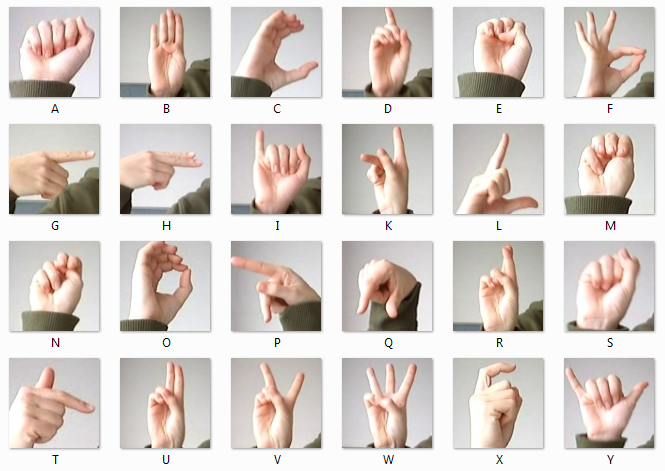
\includegraphics[width=3.4in]{figures/amer_sign2}
	\caption[]{Image of each signed letter in the dataset} %\label{American_Sign} 
\end{figure}



\section{Literature Review} \label{lit_rev}

Convolutional neural networks are able to interpret images with spatial context intact. They scan an image left to right with a small, focused window frame, typically 3x3 or 5x5 pixels, processing the features in each section. As it scans through the entire image extracting important features hierarchically, the model is able to piece together what is in the picture with high accuracy. 

Simplistically, a dense layer is able to learn a holistic pattern in the image, while a convolutional layer is able to learn local patterns within an image. Once the convolutional layer learns a pattern in one area of the picture, it will be able to find that same pattern anywhere in an image  \citep{chollet}. 

The convolutional layer will use many different filters scanning through the image over and over again. There may be one filter that is searching for horizontal lines, another focused on vertical lines, and another searching for arches. The features detected through the filters are then combined into a feature map. There will be many different feature maps created within a single convolutional layer.

Figure 2 illustrates the makeup of a simple convolutional neural network model. The first several layers focus on feature extraction from the input data. During the feature extraction process there are many feature maps visible. As the flow moves from Conv\_1 to Max-pooling, there is a compression of data. This model funnels the features from left to right until it reaches a manageable number for the final layers with only the most impactful features. The model concludes by flattening out the last convolutional layer to flow into a densely connected final layer with the classification of the image as its output.


\begin{figure}[!h] 
    \centering
	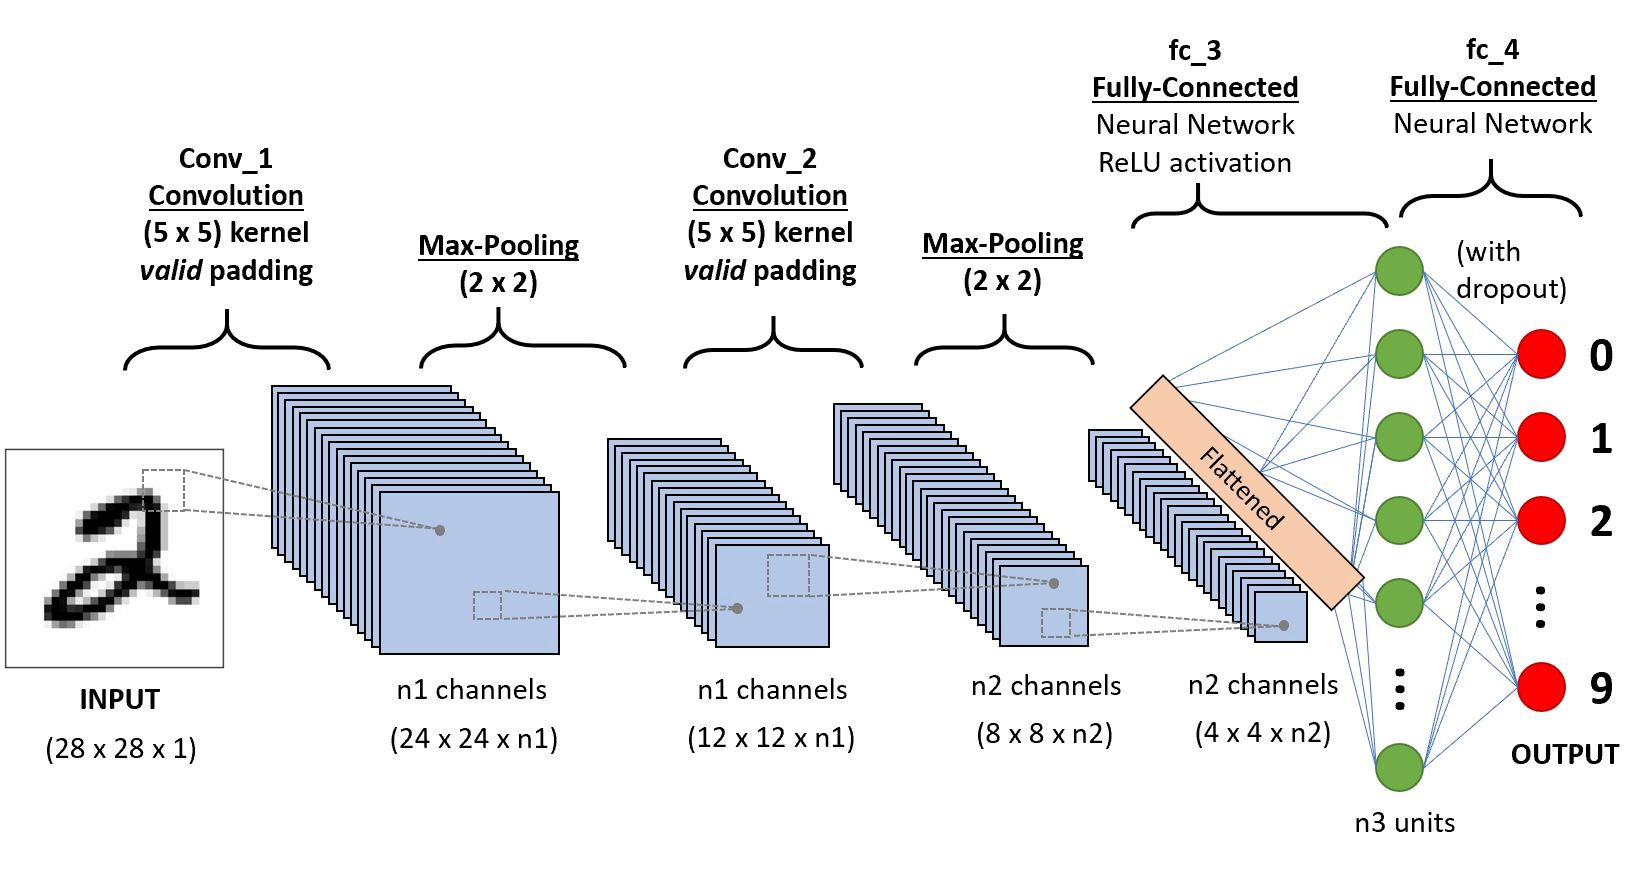
\includegraphics[width=3.4in]{figures/ConvNet.jpeg}
	\caption[]{Convolutional Neural Network Model} 
	\label{ConvNet} 
\end{figure}



\subsection{Convolutional Layer}

Convolutional layers ingest three-dimensional data: image height, image width, and channel; color images have three channels, while black and white images only have one. The convolutional layer uses a window that slides left to right across the image using filters, or kernels, that extract features from the window and place them onto the output feature map. Figure 3 shows how this process occurs. The number of pixels the window slides is known as the stride.

\begin{figure}[!h] 
    \centering
	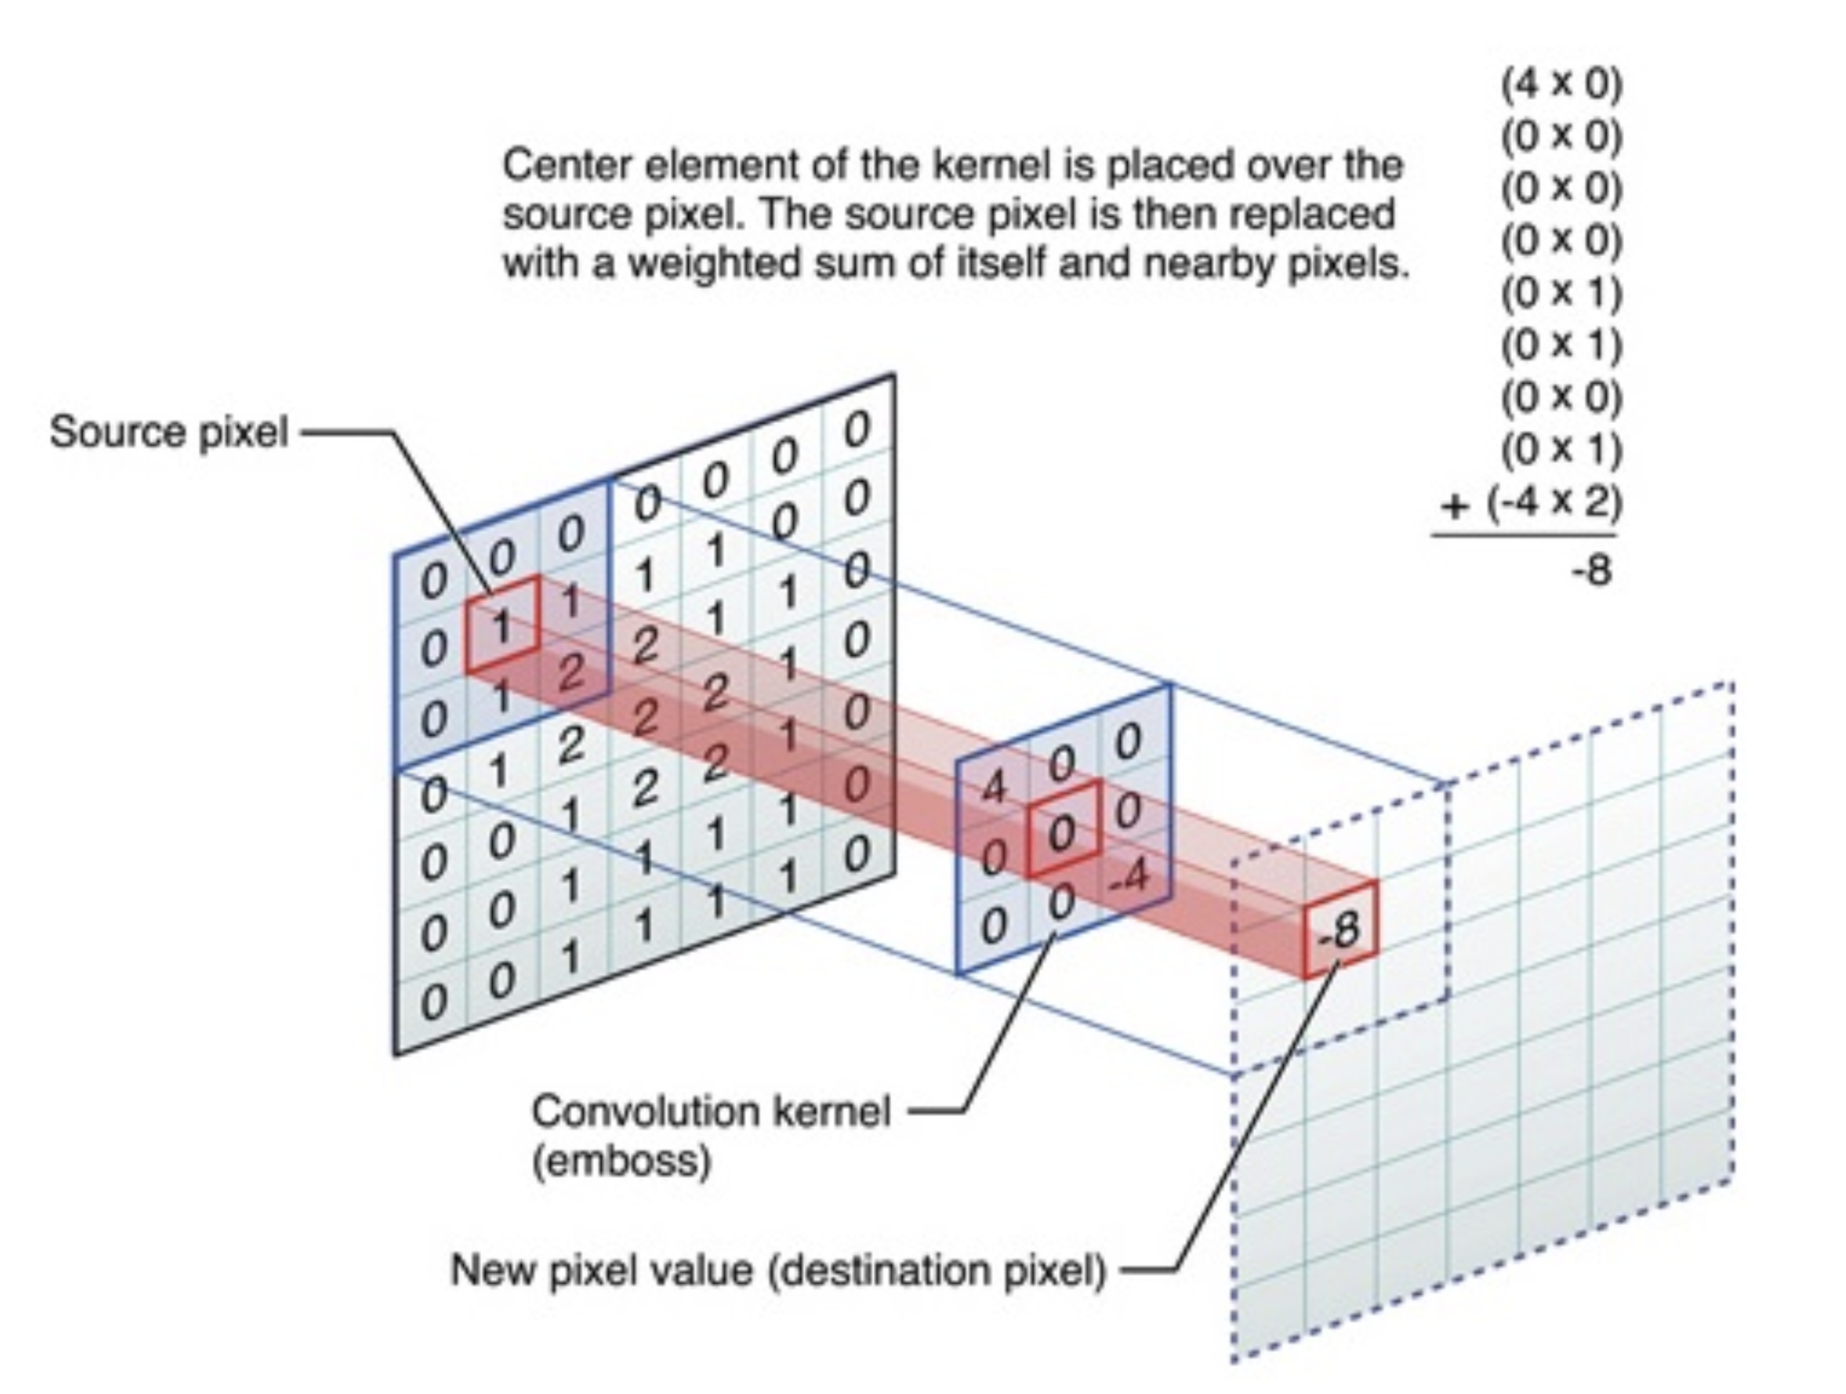
\includegraphics[width=3.4in]{figures/Conv-Layer.png}
	\caption[]{Example of convolutional layer filter, or kernel, extracting a feature within the first window frame} 
	\label{ConvNet} 
\end{figure}



A higher stride correlates to greater compression, while a smaller stride will produce less compression. Window size and stride should be considered together as a ratio. Common settings are either 5x5 or 3x3 window size and a three or two pixel stride respectively. This will create some overlap in the window frames, which will allow the filters to find features that may be found on the edges of a given window.

\subsection{Pooling Layer}

Pooling layers are used to compress the size of the image. Small sections of the image are boiled down into a single output. If the frame size was 5x5 pixels there would be 25 total pixels. The entire window of 25 pixels would be compressed into a single pixel and passed to the next layer in the neural network.  

Max pooling is the most common but there are other types of pooling layers that can used like mean pooling. That single pixel passed onto the next layer will be the maximum value in the 5x5 frame if a max pooling layer was used. It would be the average value if a mean pooling layer was used. Figure 4 provides a visual representation of how a 2x2 section is compressed into one pixel.  

\begin{figure}[!h] 
    \centering
	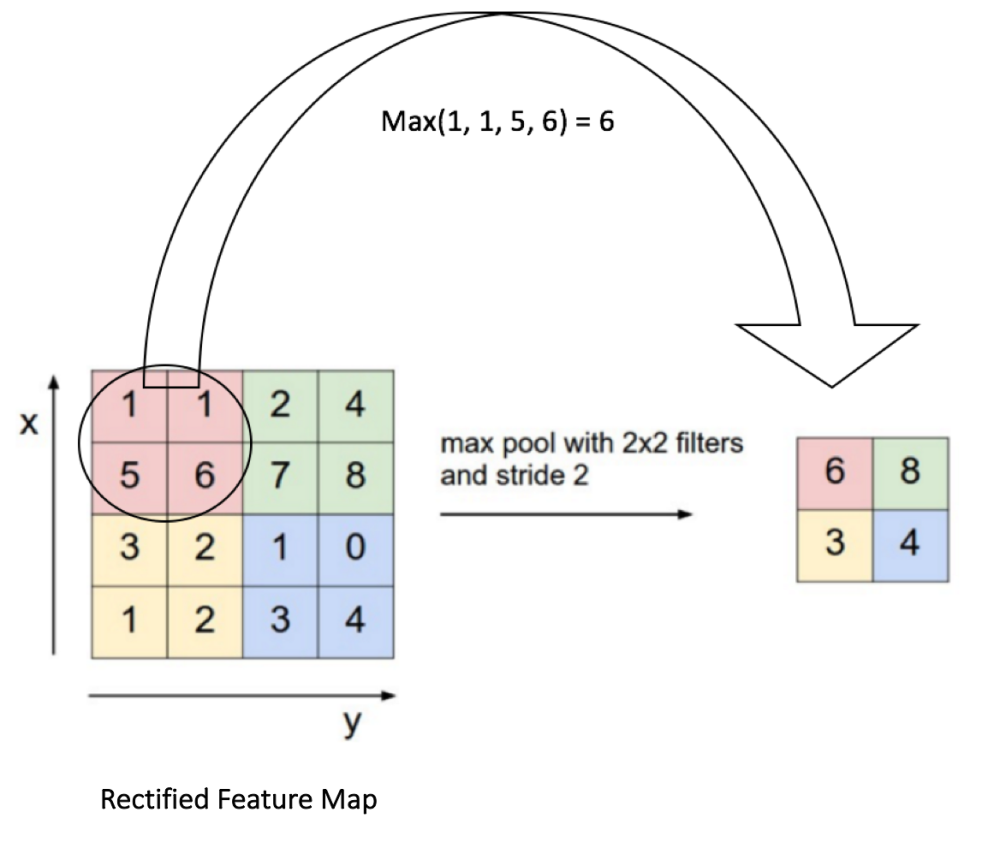
\includegraphics[width=3.4in]{figures/Max-Pooling.png}
	\caption[]{Example of how a max pooling layer compresses a 2x2 pixel window into a single pixel} 
	\label{MaxPool} 
\end{figure}

Using pooling layers in convolutional neural networks will allow them to more accurately predict an image when it is not in its perfect form \citep{brownlee}. For example, if an image is blurry or has some variation in its scale, the pooling layer will help the algorithm interpret the image properly fixing the problem. 


\subsection{Dropout Regularization}


Convolutional neural networks can easily fall into a trap where they actually memorize the training dataset, known as overfitting. This will make the model ineffective when trying to predict on never before seen observations. To help mitigate this issue, bias and nonlinear activation functions should be used allowing the model to generalize and adapt to new incoming data \citep{brownlee1}. There is another powerful technique available for data scientists when tuning their neural networks called dropout regularization.


Dropout regularization is a process that randomly sets a proportion of internal weights to zero, “dropping” their effect from the model. As the training progress cycles through each batch and each epoch, the model has the same network parameters but each batch of data will encounter a new network architecture. The randomization of weights dropped allows the model to be more robust according to \citep{albon}. Nodes within a neural network have a tendency to rely too heavily on their neighboring node’s weight. \cite{brownlee} explains that by randomly removing different nodes each pass, the nodes are able to extract more signal instead of noise within the training dataset.


\begin{figure}[!h] 
    \centering
	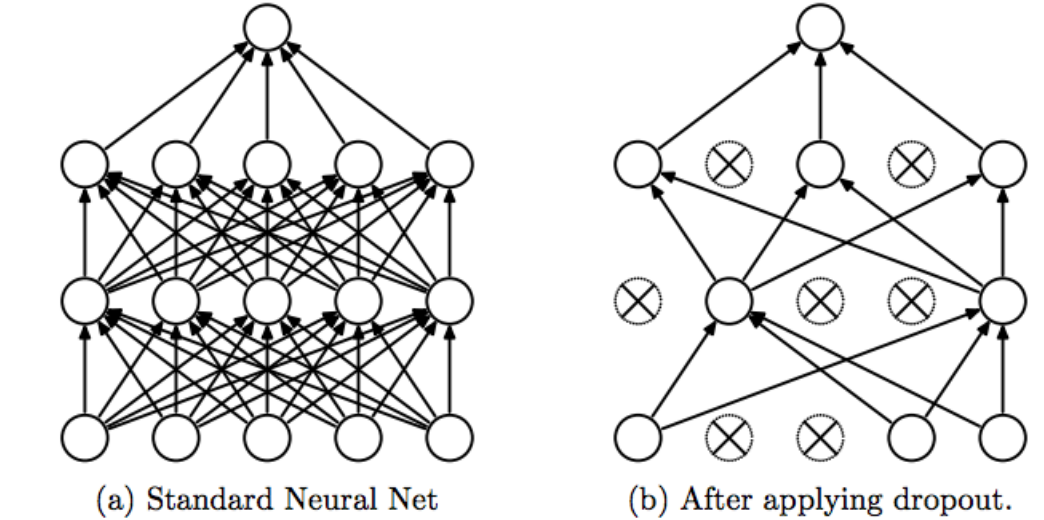
\includegraphics[width=3.4in]{figures/Dropout.png}
	\caption[]{Comparison of neural networks with and without a dropout regularization layer} 
	\label{dropout} 
\end{figure}


The suggested dropout percentage is between 20-50\%. Setting the dropout proportion to more than 50\% of the weights to zero during the training process will result in too generalized of a model missing predictive signal within the dataset. On the other hand, setting the dropout percentage to less than 20\% will have a negligible impact on the overall predictiveness of the model \citep{brownlee}.    

\section{Methodology}

The methodology undertaken in this analysis is as follows. There will be four distinct convolutional neural networks trained. Two of the models will include dropout regularization layers and two will not. There will also be two models that will incorporate back to back convolutional layers within the network structure. Using these four models, there will be an apples-to-apples comparison on whether the dropout layer and the back-to-back convolutional layers are beneficial to include when building deep learning computer vision models. 

Everything else between the four models will be congruent. The mini batch size for each model’s training will be fixed at 82. The optimization function and loss function will also be consistent across all of the models. 

The Keras package in Python, which is built on TensorFlow, will be used to develop each of the four deep neural networks. The training process for each neural network will run for a total duration of 10 epochs. Each convolutional and dense hidden layer will use a rectified linear unit (ReLU) activation function and the output layer will use the softmax activation function.



\subsection{Neural Network Architecture}

There will be four convolutional neural networks trained in this study. There will be two different core structures. Within each structure there will be two different models built, one including dropout layers and the other without. Each neural network will conclude with a flattening process before a fully connected, or dense, layer. This single dense layer will be connected to the output layer. 

\subsubsection{Layers}

There are four different neural network topology variations in this study: \\


1.	CNN-1 will have 11 steps in its model with 3,300,634 total trainable parameters:

\begin{enumerate}
 \item Input Layer
 \item Convolutional Layer - (1,644 parameters)
 \item Pooling Layer
 \item Dropout - 25\%
 \item Convolutional Layer - (73,856 parameters)
 \item Pooling Layer
 \item Dropout - 30\%
 \item Flatten
 \item Dense Layer - (3,211,776 parameters)
 \item Dropout - 50\%
 \item Output Layer - (13,338 parameters)
\end{enumerate} \\



2.	CNN-2 will have 8 steps in its model with 3,300,634 total trainable parameters: 

\begin{enumerate}
 \item Input Layer
 \item Convolutional Layer - (1,644 parameters)
 \item Pooling Layer
 \item Convolutional Layer - (73,856 parameters)
 \item Pooling Layer
 \item Flatten
 \item Dense Layer - (3,211,776 parameters)
 \item Output Layer - (13,338 parameters)
\end{enumerate} \\


3.	CNN-3 will have 13 steps in its model with 3,550,682 total trainable parameters:

\begin{enumerate}
 \item Input Layer
 \item Convolutional Layer - (1,644 parameters)
 \item Convolutional Layer - (102,464 parameters)
 \item Pooling Layer
 \item Dropout - 25\%
 \item Convolutional Layer - (73,856 parameters)
 \item Convolutional Layer - (147,584 parameters)
 \item Pooling Layer
 \item Dropout - 30\%
 \item Flatten
 \item Dense Layer - (3,211,776 parameters)
 \item Dropout - 50\%
 \item Output Layer - (13,338 parameters)
\end{enumerate} \\


4.	CNN-4 will have 10 steps in its model with 3,550,682 total trainable parameters:

\begin{enumerate}
 \item Input Layer
 \item Convolutional Layer - (1,644 parameters)
 \item Convolutional Layer - (102,464 parameters)
 \item Pooling Layer
 \item Convolutional Layer - (73,856 parameters)
 \item Convolutional Layer - (147,584 parameters)
 \item Pooling Layer
 \item Flatten
 \item Dense Layer - (3,211,776 parameters)
 \item Output Layer - (13,338 parameters)
\end{enumerate} \\




\subsubsection{Optimization Function}

The optimization function used for all of the neural networks will be the Adaptive Moment Estimation (Adam) optimizer in the Keras’ package. The Adam optimization method implements aspects from both the RMSProp and Momentum methods.  

The Adam method computes the exponentially weighted average of past gradients as well as the exponentially weighted average of the squares of past gradients. Both of these calculations are biased towards zero. The Adam optimizer performs a slight adjustment to correct the bias. Then the parameters in the model are updated \citep{adam}. 



\subsubsection{Loss Function}

The loss function employed in each deep neural network for this study is the categorical cross-entropy function because there are 26 categorical outcomes in the model. The categorical cross-entropy method explained by \cite{mool} follows the form:

$$Loss = -\sum_{i}^n y_i \log_2 y_i$$

\subsection{Dataset}

The dataset, obtained through \cite{kaggle} and inspired by the MNIST digit and fashion datasets, contains 34,627 images with the hand gesture for each letter in the American Sign language alphabet. There will only be 24 classes predicted in the model instead of 26 because the letters J and Z require motion. The images will contain a cropped signed letter in different settings. Figure \ref{Random Samples} contains 9 random sample images within the dataset in the form the model will ingest the images.


\begin{figure}[!htb] \centering
	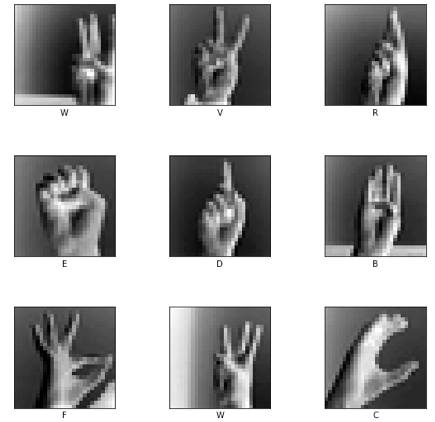
\includegraphics[width=3.4in]{figures/9-random-samples.png}
	\caption[]{9 Random Sample images} 
	\label{Random Samples} 
\end{figure}


This dataset was expanded by slight modifications of orientation by 3 degrees, random pixilation, and +/- 15\% adjustment to the brightness/contrast. These image augmentations will provide the model imperfect samples to learn, helping lower the variation when predicting on new images. A visual example of these augmentations for the letter “D” is found in Figure \ref{American_Sign}.

\begin{figure}[!htb] \centering
	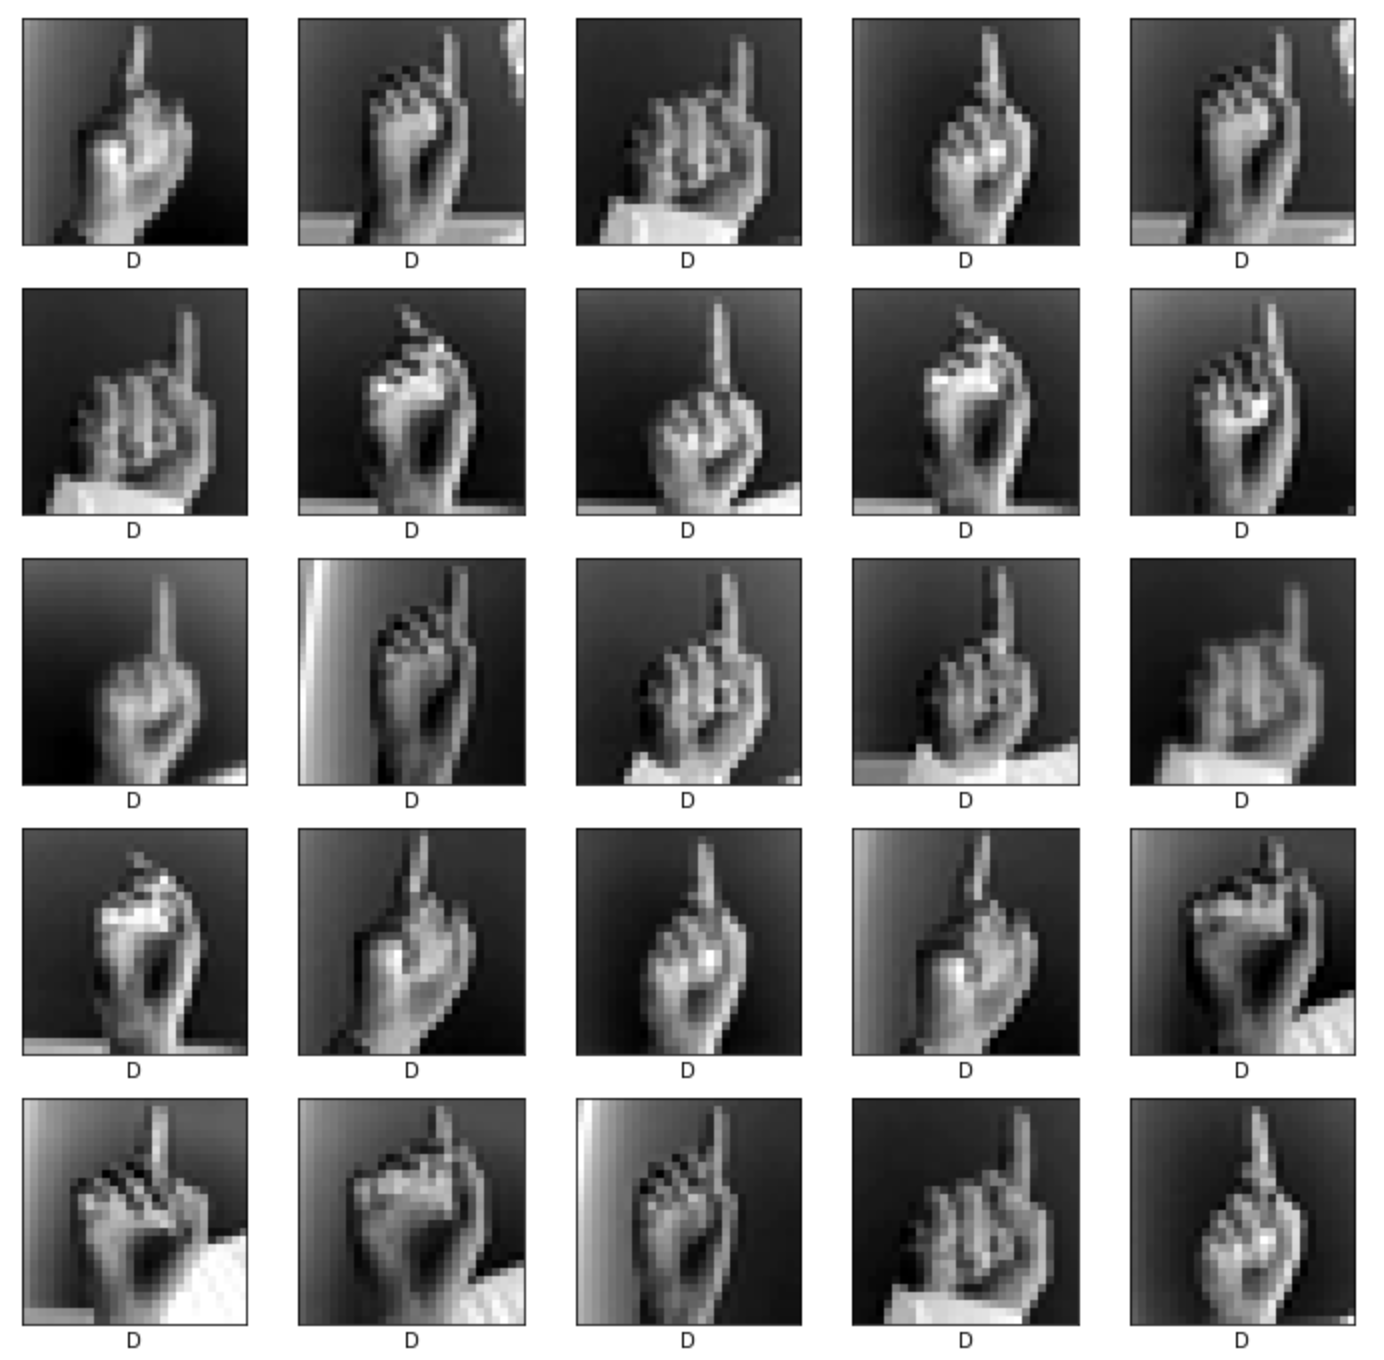
\includegraphics[width=3.4in]{figures/Sign-Language-D.png}
	\caption[]{25 sample images showing the data augmentations for the letter D} 
	\label{American_Sign} 
\end{figure}


The dataset will be split into training, validation, and testing datasets at a 64-16-20 proportion. Using 80\% of the dataset for the training and validation process will provide our neural networks enough data to learn the subtle differences between each hand gesture. The 20\% reserved for testing will provide a completely unseen dataset to determine which of the four models would perform the best in the real world. These data splits will help combat the issue of overfitting.

Each observation in the dataset has been transformed and split into input variables – pixels – and a target variable – letter label – to feed into the neural networks.  


\subsubsection{Input Data}

The images in the dataset are sized at 28x28 pixels, giving the model 784 total features. Each of the 784 features is a grayscale value between 0-255. These grayscale values will be divided by 255 to provide the neural network with scaled inputs. This feature transformation will improve the overall performance of the model. 

The shape of the input data into the convolutional neural networks will be a three-dimensional array (28, 28, 1) for the image height, image width, and channel respectively. 


\subsubsection{Target Data}

This particular modeling scenario is a classification problem. The target variable is a categorical variable with 26 different classes, one for each letter in the alphabet. Even though there are only going to be 24 letters in this dataset, 26 classes will be used to provide consistency with the previous study \citep{jason}. Each observation will represent a class label ranging from 0 to 25. There will be no observations for classes 9 and 25 because of the motion involved in signing the letters, as they map to J and Z respectively.


\section{Computational Experiment and Results}

The entire Python code for this analysis can be reproduced using Google Collaboratory Notebook at this url:\\

\href{https://colab.research.google.com/drive/10ejuNMf8NtyPXp5em7h-BDD0HYWerJeA}{Google Notebook Link} \\


The Python Notebook walks through each step from importing the data, building each convolutional neural network, and evaluating the results.   \\



\subsection{Convolutional Neural Network 1 - (CNN-1)}

The first convolutional neural network (CNN-1) has 2 sets of convolutional layers. Each convolutional layer is followed by a max pooling layer to reduce the number of features and then has a dropout layer to decrease the likelihood of overfitting on the input data. Figure \ref{CNN-1 Model Summary} gives a summary of the model with the total number of parameters updated during the training process. It also shows the order and shape of the data as it flows through each layer until it reaches the final output layer to make the prediction.

\begin{figure}[!htb] \centering
	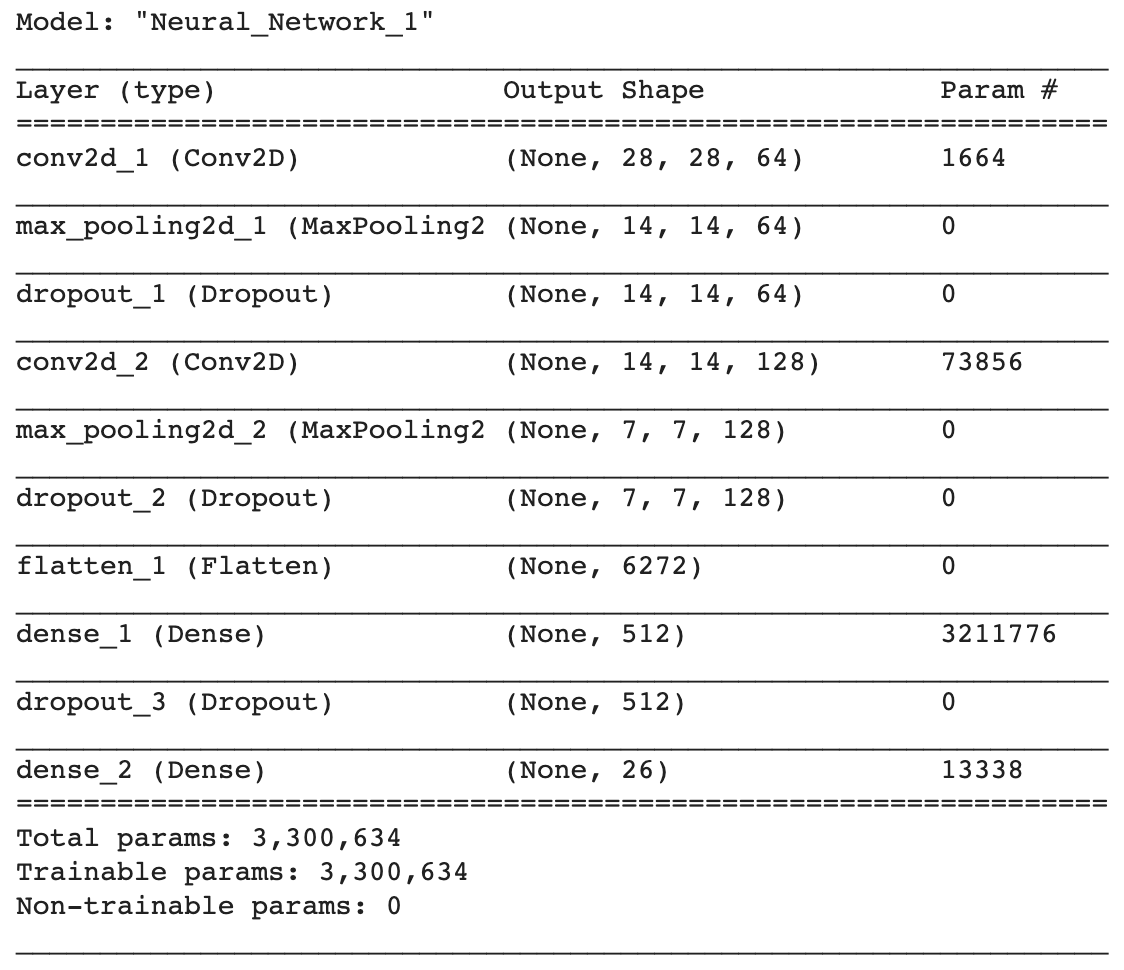
\includegraphics[width=3.4in]{figures/CNN-1-Summary.png}
	\caption[]{CNN-1 Model Summary} 
	\label{CNN-1 Model Summary} 
\end{figure}


\begin{figure}[!htb] \centering
	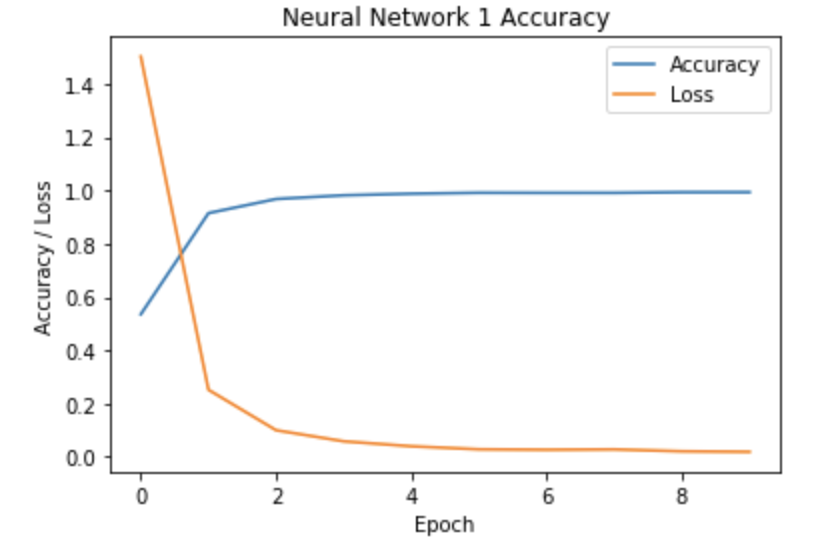
\includegraphics[width=3.4in]{figures/CNN-1-training.png}
	\caption[]{CNN-1 model Training Results} 
	\label{CNN-1 model Training Results} 
\end{figure}


Figure \ref{CNN-1 model Training Results} shows the cost/loss and accuracy of this model as it was trained over the 10 epochs. The CNN-1 model reached a maximum accuracy of 99.38\% on the training dataset and 100\% accuracy on the validation dataset over the course of 10 epochs. This model had a total training time of 15 minutes and 16 seconds.  


\subsection{Convolutional Neural Network 2 - (CNN-2)}

The second convolutional neural network (CNN-2) trained follows the same structure as CNN-1 except there will not be any dropout layers. This will allow us to have a side by side comparison of CNN-1 and CNN-2 to determine whether including dropout layers is advantageous with this computer vision problem. Figure \ref{CNN-2 Model Summary} shows each step in the model. Without the three dropout layers, there are only 8 steps from start to finish but the total number of trainable parameters are still the exact same.


\begin{figure}[!htb] \centering
	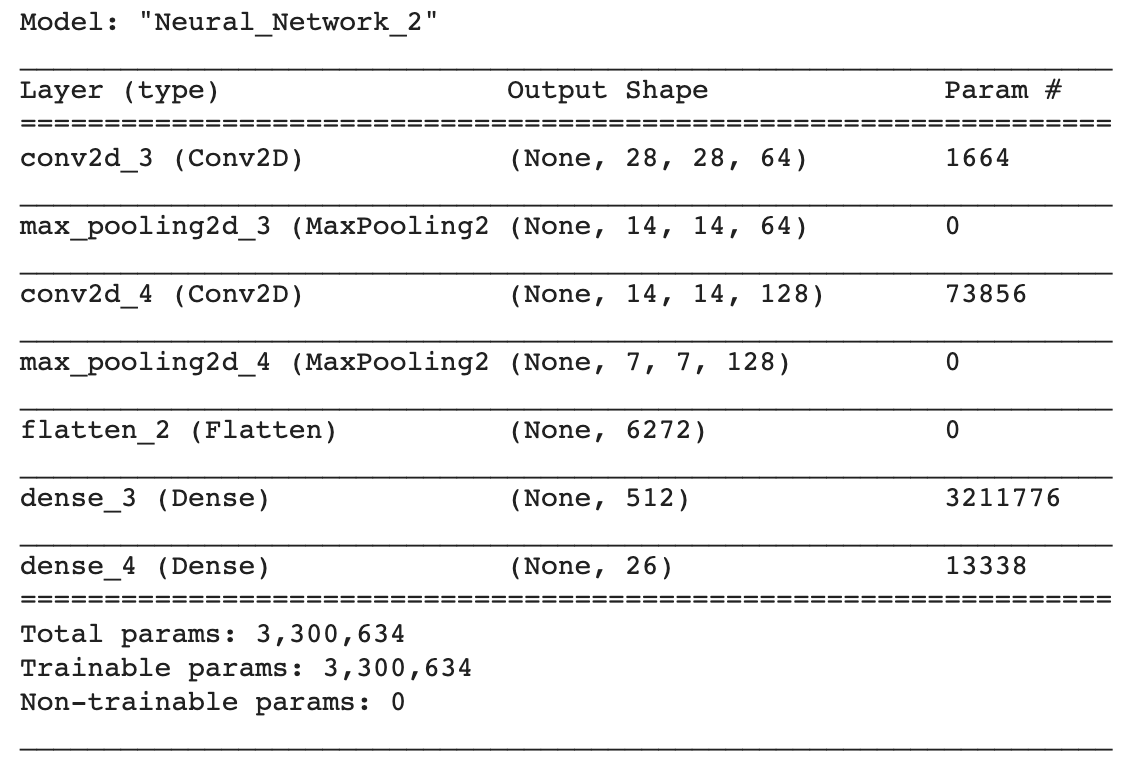
\includegraphics[width=3.4in]{figures/CNN-2-Summary.png}
	\caption[]{CNN-2 Model Summary} 
	\label{CNN-2 Model Summary} 
\end{figure}


\begin{figure}[!htb] \centering
	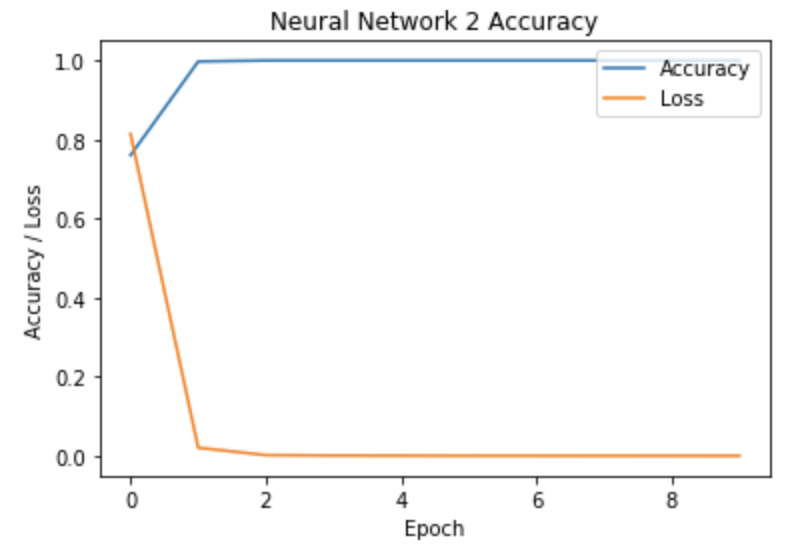
\includegraphics[width=3.4in]{figures/CNN-2-training.png}
	\caption[]{CNN-2 model Training Results} 
	\label{CNN-2 model Training Results} 
\end{figure}


Without any dropout layers, this model was able to achieve 100\% accuracy on the training dataset in only two epochs as seen in Figure \ref{CNN-2 model Training Results}. The model is able to, in a sense, memorize the training data extremely quick. This may appear to be impressive now, but it could easily cause issues with the model's performance on out-of-sample observations. 

This model decreased the training time by 5\% compared to its counterpart model CNN-1. Removing the dropout layers was able to save training time. The total training time for the 10 epochs was 14 minutes and 30 seconds 


\subsection{Convolutional Neural Network 3 - (CNN-3)}


The third convolutional neural network (CNN-3) has an extra convolutional layer added directly after the preceding convolutional layer. Building a network with back to back convolutional layers increases the training time dramatically. However, this will allow the model to extract higher level features within the image. Figure \ref{CNN-3 Model Summary} provides a summary of the model with the total number of layers.


\begin{figure}[!h] 
    \centering
	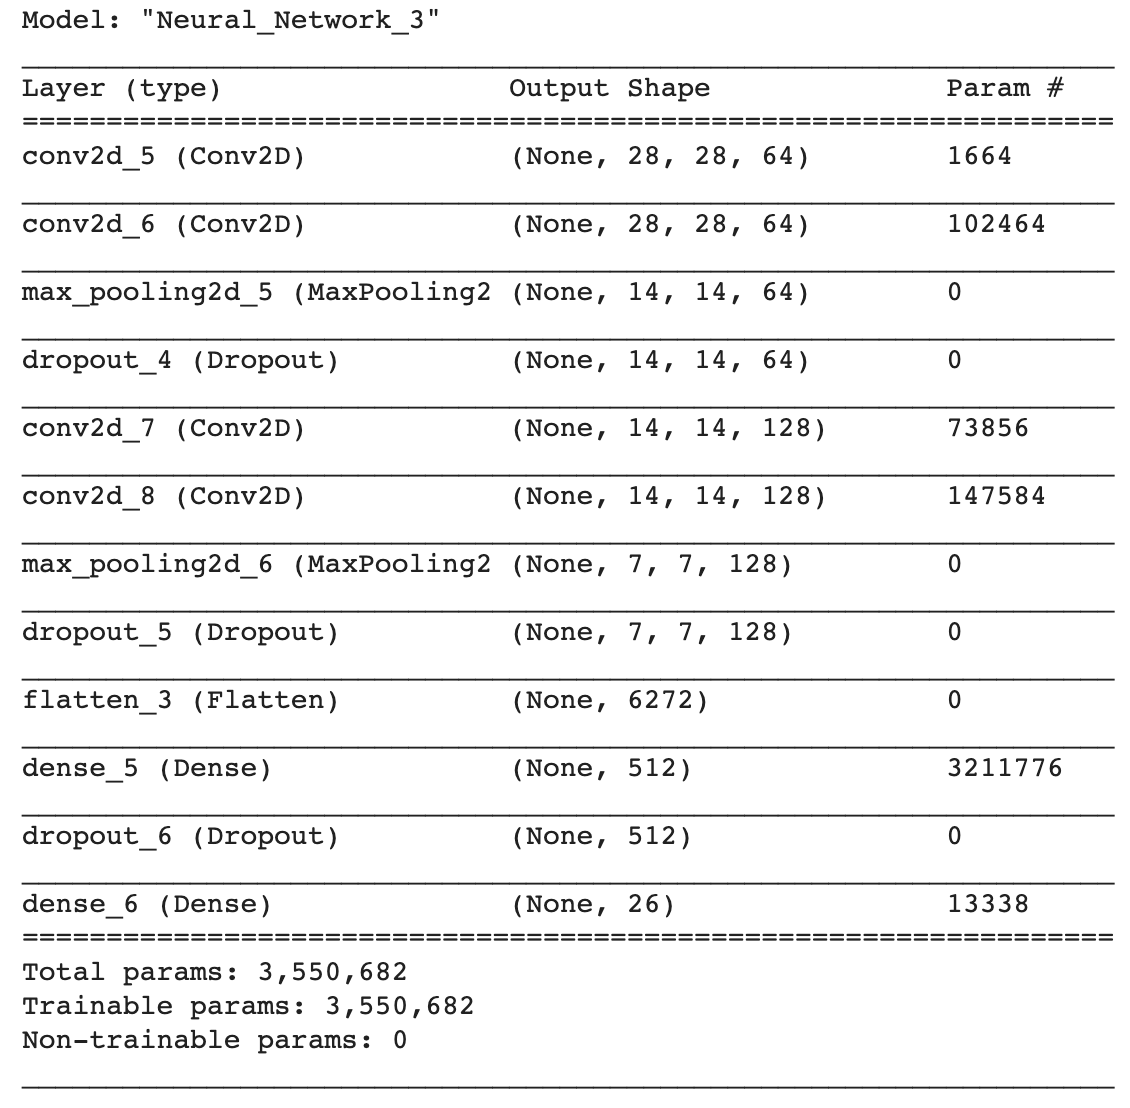
\includegraphics[width=3.4in]{figures/CNN-3-Summary.png}
	\caption[]{CNN-3 Model Summary} 
	\label{CNN-3 Model Summary} 
\end{figure}


\begin{figure}[!htb] \centering
	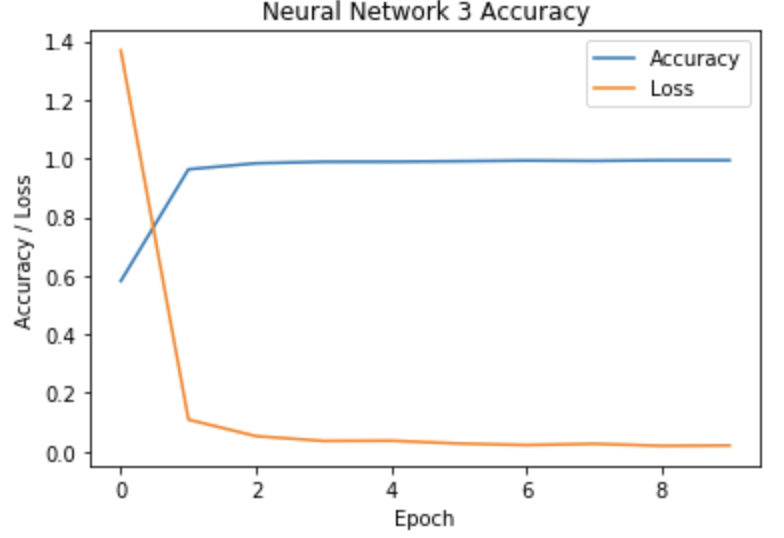
\includegraphics[width=3.4in]{figures/CNN-3-training.png}
	\caption[]{CNN-3 model Training Results} 
	\label{CNN-3 model Training Results} 
\end{figure}


As can be seen in Figure \ref{CNN-3 model Training Results}, this model reached a maximum accuracy of 99.36\% on the training dataset and 100\% accuracy on the validation dataset over the course of 10 epochs. This model’s training time was 1 hour 15 minutes and 37 seconds.



\subsection{Convolutional Neural Network 4 - (CNN-4)}


The fourth and final convolutional neural network (CNN-4) has the same structure as CNN-3 but without the dropout layers. There are 3,550,682 trainable parameters in this model, consistent with CNN-3. These two models will be used as side by side comparisons. The steps and layers are shown in Figure \ref{CNN-4 Model Summary}.


\begin{figure}[!htb] \centering
	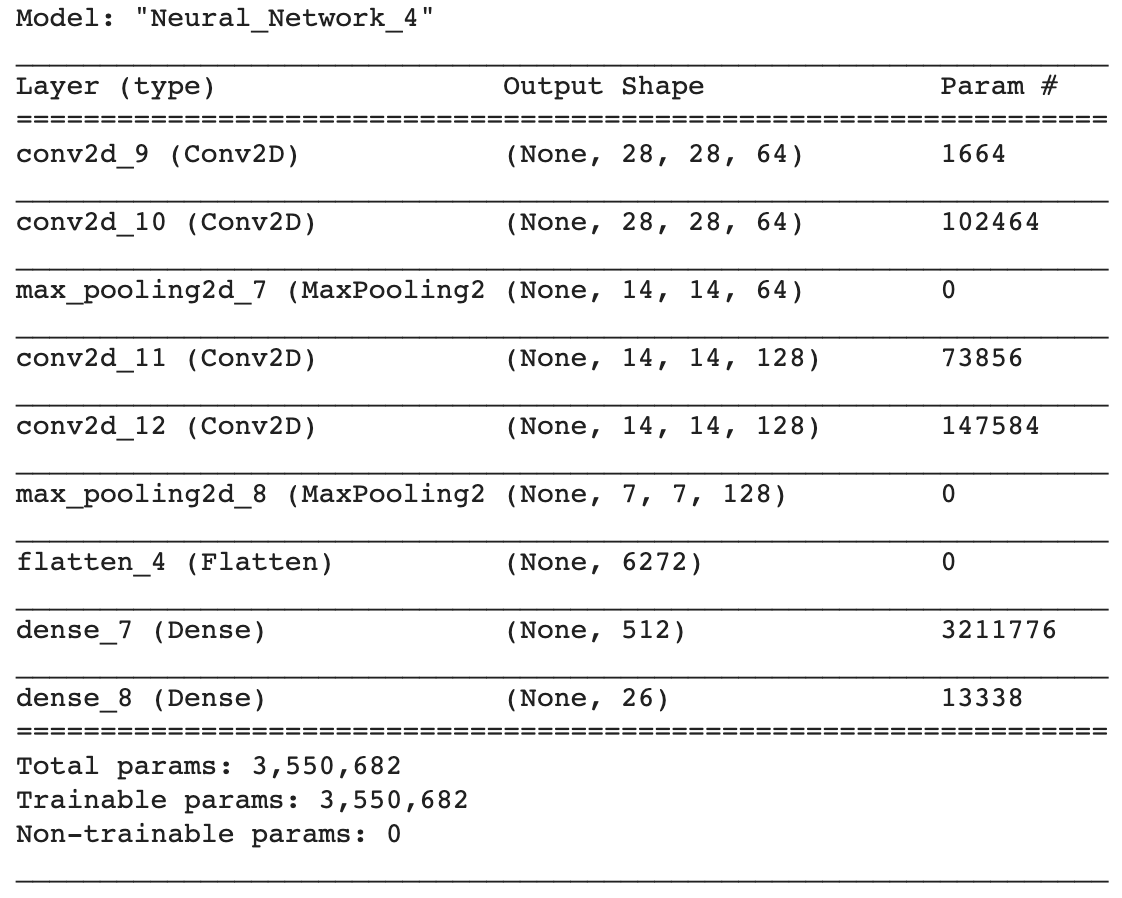
\includegraphics[width=3.4in]{figures/CNN-4-Summary.png}
	\caption[]{CNN-4 Model Summary} 
	\label{CNN-4 Model Summary} 
\end{figure}


\begin{figure}[!htb] \centering
	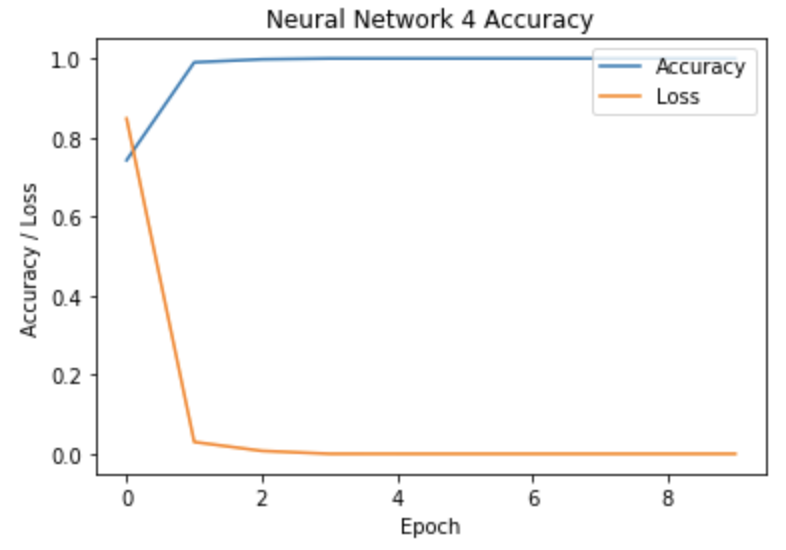
\includegraphics[width=3.4in]{figures/CNN-4-training.png}
	\caption[]{CNN-4 model Training Results} 
	\label{CNN-4 model Training Results} 
\end{figure}


As can be seen in Figure \ref{CNN-4 model Training Results}, this model reached a maximum accuracy of 99.36\% on the training dataset and 100\% accuracy on the validation dataset over the course of 10 epochs. This model’s training time was 1 hour 15 minutes and 35 seconds, only 2 seconds quicker than CNN-3.

\section{Discussion and Conclusions}


\begin{figure}[!htb] \centering
	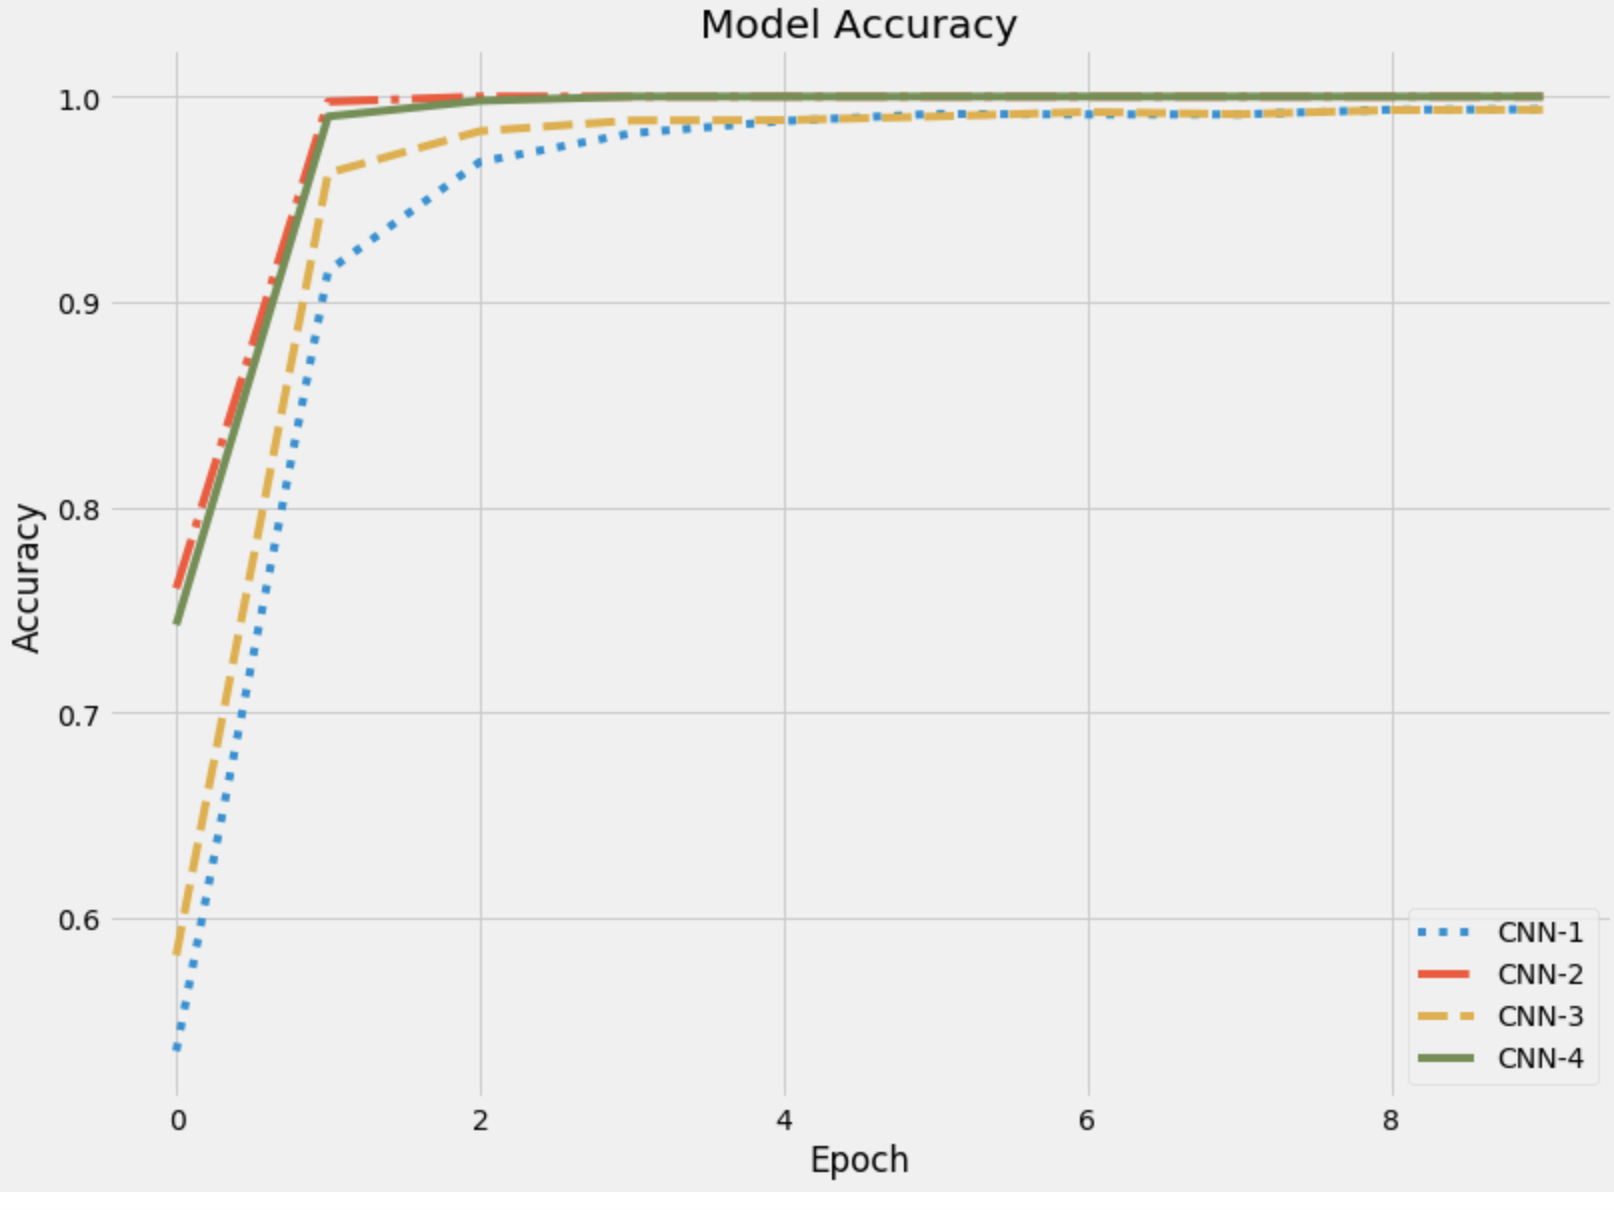
\includegraphics[width=3.4in]{figures/Model-Accuracy-Evaluation.png}
	\caption[]{Accuracy Comparison between the 4 models} 
	\label{Accuracy} 
\end{figure}


\begin{figure}[!htb] \centering
	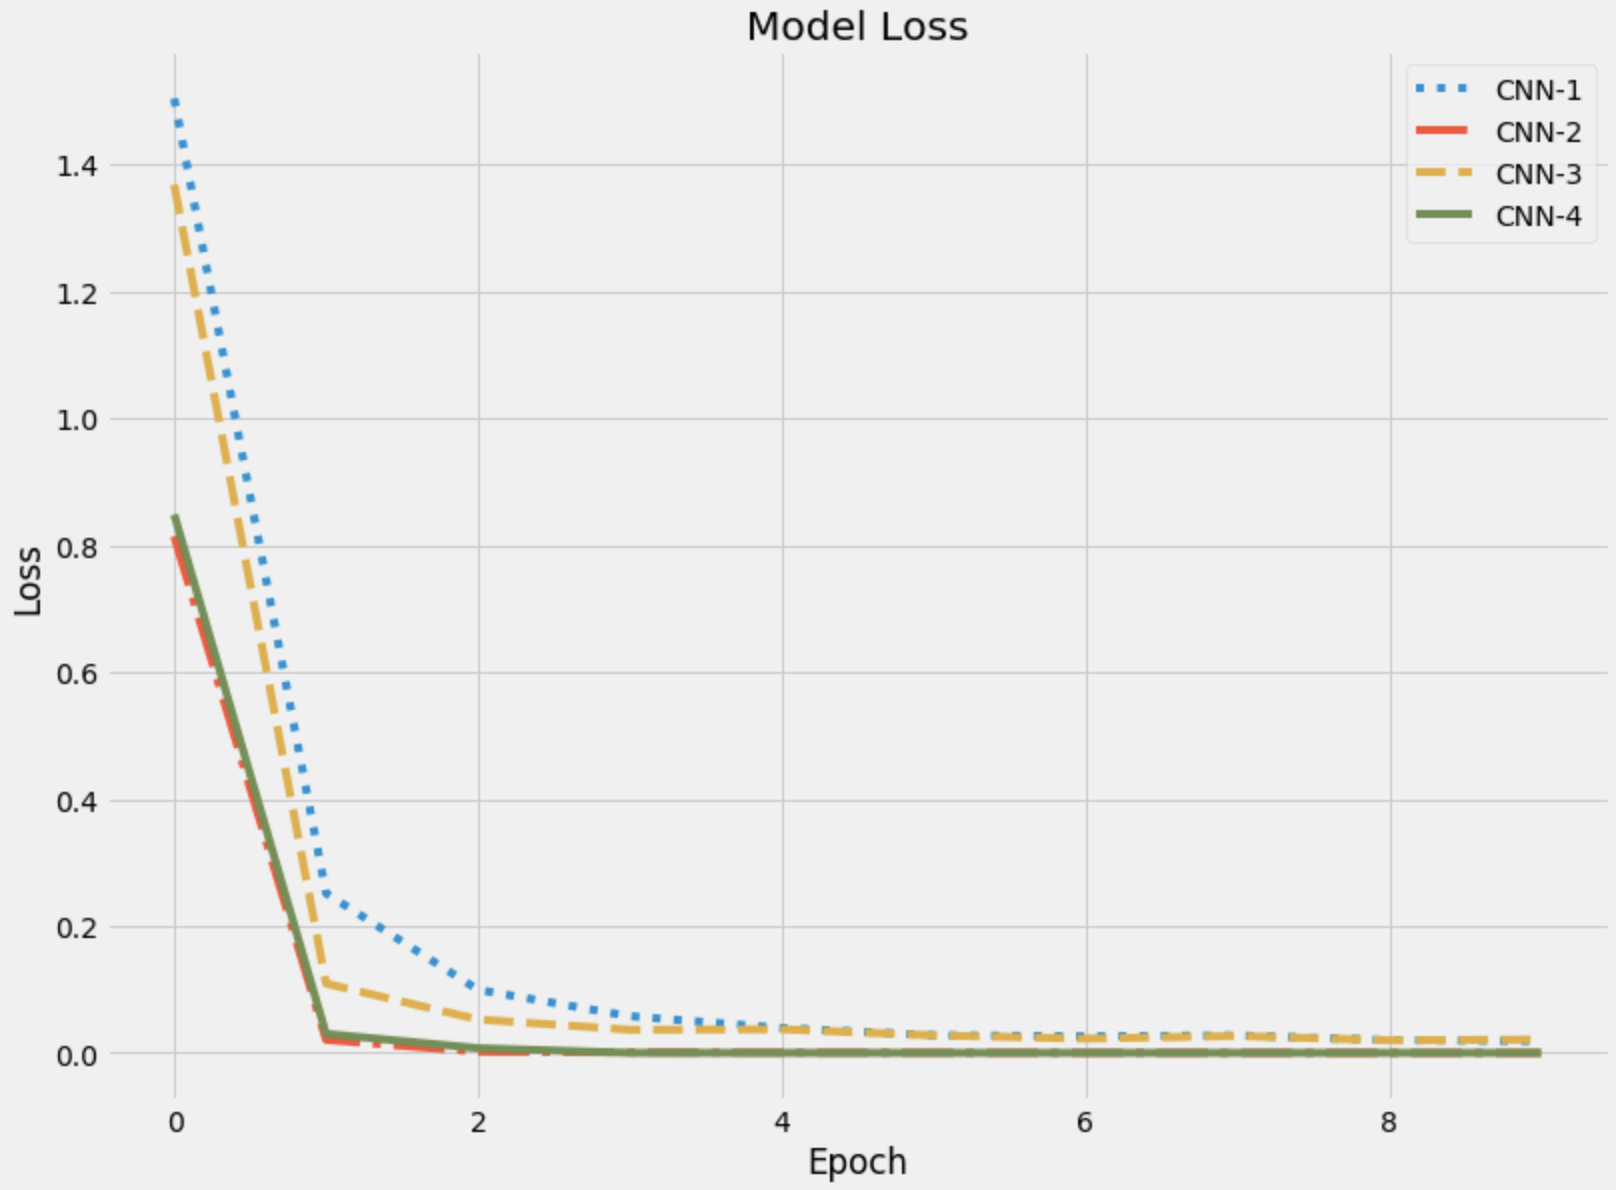
\includegraphics[width=3.4in]{figures/Model-Loss-Evaluation.png}
	\caption[]{Loss/Cost Comparison between the 4 models} 
	\label{Loss} 
\end{figure}


\begin{table}[!htb] 
  \centering 
  \begin{tabular}{@{\small}llll@{}} 
    \toprule % utilise booktabs
    & {\footnotesize Training Time} &  {\footnotesize Validation Accuracy} & {\footnotesize Test Accuracy} \\ \midrule
    CNN-1 & 15:16 & 100\% & 93.95\% \\
    CNN-2 & 14:30 & 100\% & 92.47\% \\
    CNN-3 & 1:15:37 & 100\% & 95.58\% \\
    CNN-4 & 1:15:35 & 100\% & 92.76\% \\ 
    \bottomrule
\end{tabular} \caption{Side by Side comparison of the four Convolutional neural networks} \label{table_eval}
\end{table}


Each convolutional neural network trained during this study accomplished the overall learning task to recognize each letter in the American Sign Language alphabet with over 100\% accuracy on the validation dataset. However, only CNN-3 was able to achieve over 95\% on the test dataset. This gives credence to the importance of using dropout regularization techniques to avoid overfitting and using multiple convolutional layers to extract higher level features in the data.

The side by side comparison for the benefit of using dropout layers seen when looking at CNN-1 vs CNN-2 and CNN-3 vs CNN-4 shows that there is a lift when including the dropout layers. 

The side by side comparison for the benefit of using back to back convolutional layers seen when looking at CNN-1 vs CNN-3 and CNN-2 vs CNN-4 shows that there is also a lift when including the back to back convolutional layers. However, the training time increased by almost 400\%. Convolutional neural networks are one of the most computationally expensive algorithms and it is advised to have the proper hardware when training these models.

It is extremely convoluted trying to decipher exactly what is going on inside “black-box” algorithms, like deep neural networks. There will always be limitations with modeling, like statistician George Box says, “All models are wrong, but some are useful” \citep{box}. Understanding what each layer adds to the model and how the different layers, methods, and techniques can impact the results will allow data scientists to confidently deploy deep neural networks in the real world. 



\section*{Appendix}


\bibliography{bibliographie.bib}

\bibliographystyle{newapa}

\end{document}